%! Author = ryanb
%! Date = 10/31/2025

% Preamble
\documentclass{amsart}

% Packages
\usepackage{amsmath}
\usepackage{amsrefs}
\usepackage{amsthm}

\usepackage{tikz}
\usepackage{float}

\usepackage{hyperref}
\usepackage{wrapfig}
\usepackage{mathtools}

\usetikzlibrary{backgrounds}

\theoremstyle{definition}
\newtheorem{definition}{Definition}[section]

\theoremstyle{plain}
\newtheorem{theorem}{Theorem}[section]

\newcommand{\N}{\mathbb{N}}
\newcommand{\Z}{\mathbb{Z}}
\newcommand{\Q}{\mathbp{Q}}
\newcommand{\C}{\mathbb{C}}
\newcommand{\F}{\mathbb{F}}
\newcommand{\R}{\mathbb{R}}

% Document
\begin{document}

    \title{Planar Graphs and Planarity}

    \author{Lucas Johnson}
    \author{Nathan LaCrosse}
    \author{Nick Proctor}
    \author{Ryan Bruno}

    \date{\today}

    \maketitle

    \tableofcontents % uncomment if needed

    \section{Introduction to Planar Graphs}\label{sec:intro}

    \begin{definition}
        A graph $G$ is called a \emph{planar graph} if $G$ can be drawn in the plane without any two of its edges crossing~\cite{ourBook}.
        If $G$ is already drawn in the plane without crossings, then $G$ is a \emph{plane graph}.
    \end{definition}
    Importantly, any graph isometric to a plane graph is therefore planar.
    \begin{center}
        \begin{figure}[H]
            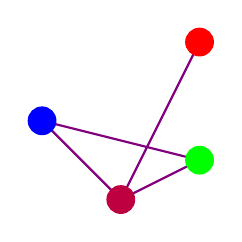
\begin{tikzpicture}[scale=0.5]
                \draw[violet, thick] (0,2) -- (2,0);
                \draw[violet, thick] (2,0) -- (4,1);
                \draw[violet, thick] (4,1) -- (0,2);
                \draw[violet, thick] (2,0) -- (4,4);

                \filldraw [blue] (0, 2) circle (10pt);
                \filldraw [purple] (2, 0) circle (10pt);
                \filldraw [green] (4, 1) circle (10pt);
                \filldraw [red] (4, 4) circle (10pt);
            \end{tikzpicture}
            \hspace{1in}
            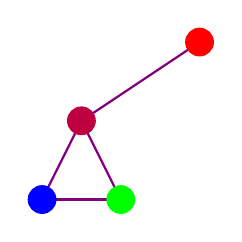
\begin{tikzpicture}[scale=0.5]
                \draw[violet, thick] (0,0) -- (2,0);
                \draw[violet, thick] (2,0) -- (1,2);
                \draw[violet, thick] (1,2) -- (0,0);
                \draw[violet, thick] (1,2) -- (4,4);

                \filldraw [blue] (0, 0) circle (10pt);
                \filldraw [purple] (1, 2) circle (10pt);
                \filldraw [green] (2, 0) circle (10pt);
                \filldraw [red] (4, 4) circle (10pt);
            \end{tikzpicture}\caption{The graph on the left is planar since it is isomorphic to the plane graph on the right.}\label{fig:isomorphicPlanar}
        \end{figure}
    \end{center}
    From here on, when referring to planar graphs, we will be considering the plane graph that the graph is isomorphic to.
    Often, when working with planar graphs, one is concerned with whether or not a given graph is planar.
    This question appears often in contexts where there are connections on a $2D$ grid and intersections are impossible.

    In order to solve this, we must discuss what properties define a planar graph.
    One important theorem is the Euler Identity.
    \begin{theorem}[The Euler Identity~\cite{ourBook}]
        For every connected plane graph of order $n$, size $m$ and having $r$ regions,
        \[n-m+r=2.\]
    \end{theorem}

    In order to be able to understand this theorem, let us first discuss the regions of a graph.
    A \emph{region} is an area bounded by the edges and vertices of a graph $G$.
    Additionally, there is an external region which is unbounded.
    \begin{figure}[H]
        \centering
        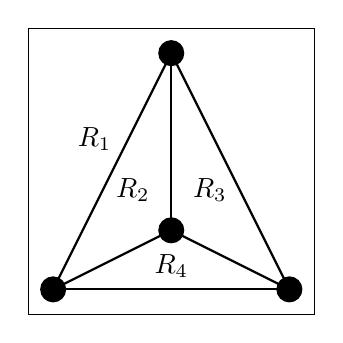
\begin{tikzpicture}[scale=0.75, show background rectangle]
            \draw[black, thick] (0,0) -- (2,4);
            \draw[black, thick] (0,0) -- (2,1);
            \draw[black, thick] (0,0) -- (4,0);

            \draw[black, thick] (2,1) -- (2,4);
            \draw[black, thick] (2,1) -- (4,0);

            \draw[black, thick] (2,4) -- (4,0);

            \filldraw [black] (2, 1) circle (6pt);
            \filldraw [black] (4, 0) circle (6pt);
            \filldraw [black] (0, 0) circle (6pt);
            \filldraw [black] (2, 4) circle (6pt);

            \node[above=0.75in, right=0.075in] at (0,0) {$R_1$};
            \node[above=0.2in, left=0.06in] at (2,1) {$R_2$};
            \node[above=0.2in, right=0.06in] at (2,1) {$R_3$};
            \node at (2,0.4) {$R_4$};
        \end{tikzpicture}
        \caption{A planar graph with its regions denoted.}
        \label{fig:regions}
    \end{figure}

    The Euler Identity is a powerful tool in characterizing planar graphs.
    However, it is difficult to determine the amount of regions in an arbitrary graph.
    Luckily, the Euler Identity leads to a result that no longer requires a region count.
    Since each edge is on the boundary of at most two regions in a graph $G$, we can use the Euler Identity to get a result in terms of the order and size of $G$.

    If $G$ is a planar graph of order $n\geq 3$ and size $m$, then
    \[m\leq 3n-6.\]
    Equivalently, if $G$ is of order $n\geq 5$ and size $m$ such that
    \[m>3n-6,\]
    then $G$ is nonplanar.

    These results lead to two important nonplanar graphs that lead to a universal planarity criterion.
    Namely, both $K_5$ and $K_{3,3}$ are nonplanar.
    $K_5$ is of order $5$ and size $20$, and since $20>15-6$, it is therefore nonplanar by our newest result.
    $K_{3,3}$ is of order $6$ and size $9$, so we can't say anything using the size formulas.
    Instead, the Euler identity requires that $6-9+r=2$.
    Therefore, $K_{3,3}$ must have $5$ regions to be nonplanar.
    However, since bipartite graphs have no odd cycles, each region of the graph requires at least four edges on the boundary (boundaries are cycles).
    Since each edge in $K_{3,3}$ is on a cycle, it is on the boundary of two regions -- so each edge gets counted twice when constructing these regions.
    Therefore, the minimum size of $K_{3,3}$ must be $\frac{5\times 4}{2}=10$.
    However, since $K_{3,3}$ is of size $9$, this is impossible~--~so $K_{3,3}$ must be nonplanar.
    \begin{figure}[H]
        \centering
        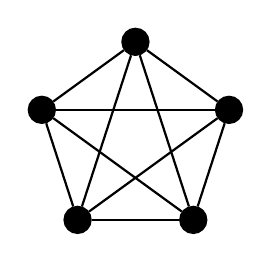
\begin{tikzpicture}[
            vertex/.style = {
                circle,
                draw,
                thick,
                fill=black,
                minimum size=1mm,
                font=\sffamily
            }
        ]
            \def\numVertices{5}
            \def\radius{1.25}
            \foreach \i in {1,...,\numVertices} {
                \node[vertex] (v\i) at ({90 - (\i - 1) * (360/\numVertices)}:\radius) {};
            }
            \draw[thick, color=black] (v1) -- (v2);
            \draw[thick, color=black] (v1) -- (v3);
            \draw[thick, color=black] (v1) -- (v4);
            \draw[thick, color=black] (v1) -- (v5);

            \draw[thick, color=black] (v2) -- (v3);
            \draw[thick, color=black] (v2) -- (v4);
            \draw[thick, color=black] (v2) -- (v5);

            \draw[thick, color=black] (v3) -- (v4);
            \draw[thick, color=black] (v3) -- (v5);

            \draw[thick, color=black] (v4) -- (v5);

        \end{tikzpicture}\hspace{1in}
        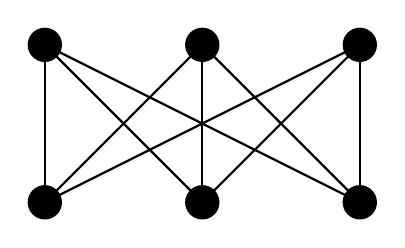
\begin{tikzpicture}
            \draw[black, thick] (0,0) -- (0,2);
            \draw[black, thick] (0,0) -- (2,2);
            \draw[black, thick] (0,0) -- (4,2);

            \draw[black, thick] (2,0) -- (0,2);
            \draw[black, thick] (2,0) -- (2,2);
            \draw[black, thick] (2,0) -- (4,2);

            \draw[black, thick] (4,0) -- (0,2);
            \draw[black, thick] (4,0) -- (2,2);
            \draw[black, thick] (4,0) -- (4,2);

            \filldraw [black] (0, 0) circle (6pt);
            \filldraw [black] (0, 2) circle (6pt);
            \filldraw [black] (2, 0) circle (6pt);
            \filldraw [black] (2, 2) circle (6pt);
            \filldraw [black] (4, 0) circle (6pt);
            \filldraw [black] (4, 2) circle (6pt);
        \end{tikzpicture}

        \caption{$K_5$ (left) and $K_{3,3}$ (right), two nonplanar graphs.}
        \label{fig:k_5k_33}
    \end{figure}

    Put simply, the idea behind the universal criterion for planarity is the following: can we show that a given graph has the same kind of geometry as $K_5$ or $K_{3,3}$?
    Furthermore, we only have to show that a part of a graph has this geometry -- as there only needs to be one instance of line crossing to have a nonplanar graph.

    To do this, we use the power of edge contractions.
    Given adjacent vertices $u$ and $v$ of a graph $G$, we define edge contraction as the process of ``merging'' the two vertices into a new vertex $w$, which is adjacent to all of the neighbors of $u$ and $v$.
    \begin{figure}[H]
        \centering
        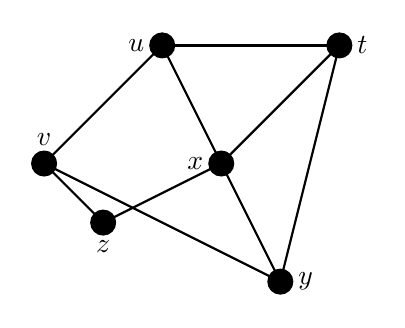
\begin{tikzpicture}[scale=0.75]
            \draw[black, thick] (0,2) -- (2,4);
            \draw[black, thick] (0,2) -- (4,0);
            \draw[black, thick] (0,2) -- (1,1);

            \draw[black, thick] (1,1) -- (3,2);

            \draw[black, thick] (4,0) -- (3,2);
            \draw[black, thick] (4,0) -- (5,4);

            \draw[black, thick] (3,2) -- (2,4);
            \draw[black, thick] (3,2) -- (5,4);

            \draw[black, thick] (2,4) -- (5,4);

            \filldraw [black] (0, 2) circle (6pt);
            \filldraw [black] (1, 1) circle (6pt);
            \filldraw [black] (4, 0) circle (6pt);
            \filldraw [black] (3, 2) circle (6pt);
            \filldraw [black] (2, 4) circle (6pt);
            \filldraw [black] (5, 4) circle (6pt);

            \node[above=3pt] at (0,2) {$v$};
            \node[below=3pt] at (1,1) {$z$};
            \node[left=3pt] at (3,2) {$x$};
            \node[right=3pt] at (4,0) {$y$};
            \node[left=3pt] at (2,4) {$u$};
            \node[right=3pt] at (5,4) {$t$};
        \end{tikzpicture}\hspace{1in}
        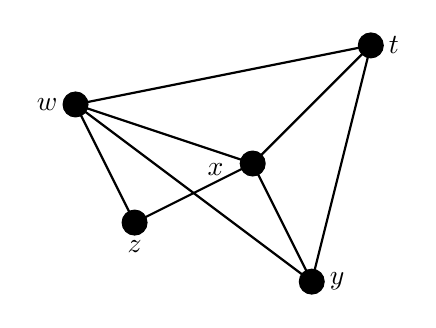
\begin{tikzpicture}[scale=0.75]
            \draw[black, thick] (1,1) -- (3,2);
            \draw[black, thick] (1,1) -- (0,3);

            \draw[black, thick] (4,0) -- (3,2);
            \draw[black, thick] (4,0) -- (5,4);

            \draw[black, thick] (3,2) -- (5,4);

            \draw[black, thick] (0,3) -- (3,2);
            \draw[black, thick] (0,3) -- (4,0);
            \draw[black, thick] (0,3) -- (5,4);

            \filldraw [black] (1, 1) circle (6pt);
            \filldraw [black] (4, 0) circle (6pt);
            \filldraw [black] (3, 2) circle (6pt);
            \filldraw [black] (5, 4) circle (6pt);
            \filldraw [black] (0,3) circle (6pt);

            \node[left=3pt] at (0,3) {$w$};
            \node[below=3pt] at (1,1) {$z$};
            \node[below=2pt, left=7pt] at (3,2) {$x$};
            \node[right=3pt] at (4,0) {$y$};
            \node[right=3pt] at (5,4) {$t$};
        \end{tikzpicture}
        \caption{A graph $G$ before and after the edge $uv$ is contracted, creating $G'$ and a new vertex $w$.}
        \label{fig:contractions}
    \end{figure}

    Any graph created by consecutively removing vertices, edges and performing edge contractions is called a \emph{minor} of the graph $G$.
    So, in the figure above, $G'$ is a valid minor of $G$.
    These minors lead into a powerful result that givs us a universal criterion for planarity.
    \begin{theorem}[Wagner's Theorem~\cite{ourBook}]
        A graph $G$ is planar if and only if neither $K_5$ nor $K_{3,3}$ is a minor of $G$.
    \end{theorem}
    In other words, if a graph $G$ can be simplified down, via vertex deletion, edge deletion, and edge contraction, into either $K_5$ or $K_{3,3}$, then it is a nonplanar graph.
    This is why proving that $K_5$ and $K_{3,3}$ were nonplanar was so important -- they are the most basic nonplanar graphs that all nonplanar graphs can be reduced to.
    This theorem and its corollaries lead to powerful results in the world of planar graphs.
    For example, there are highly efficient planarity testing algorithms that can run in linear time.

    \newpage
    \section{Planarity of Infinite Graphs}
    The graph $K_{1, n-1}$, the complete star of order n, is a graph defined as planar for all values of n.

    \subsection{Simple Construction of: $K_{1, n-1}$}
    For a graph $K_{1, n-1},\ n \geq 2$, it follows that in radial coordinates, all vertices must exist at distinct degrees.
    That is, $\left\{ \exists\ \theta_i\ \forall\ 0\leq i, k < n-1 \in \Z\ \lvert\ \theta_i \neq \theta_k \text{ and } \forall\ \theta_i, \exists\text{ radius }r_i \right\}$.
    Further, may it be assumed, for any value $n$, the distribution such that all values of $\theta_i$ are maximally spread from adjacent degrees: $\theta_{\text{mod}(i\pm 1, n-1)}$, is $\theta_i = \frac{2\pi}{n-1} i$.
    It follows, the non-origin vertices must then be:
    \[v_i = \left(r_i \cos\left(\frac{2\pi}{n-1} i\right), r_i \sin\left(\frac{2\pi}{n-1}i\right)\right);\ r_i \neq 0\]
    with edges:
    \[E\left(v_{\left(0,0\right)}, v_i\right) = \left(t\cdot r_i \cos\left(\frac{2\pi}{n-1} i \right), t\cdot r_i\sin\left(\frac{2\pi}{n-1} i\right) \right);\ 0\leq t\leq1\in \R\]
    Thus, by construction, $K_{1, n-1}$ $n$-finite is planar.
    \begin{figure}[htbp]
        \centering %\linewidth or scale=.3
        \includegraphics[height=.25\textheight]{nickScreenshot}
        \caption{$K_{1, n-1}$ of monotonically increasing radii}
        \label{fig:screenshot}
    \end{figure}

    \subsection{Planarity of $K_{1, \infty}$}
    The definition of planar requires edges to intersect only at their endpoints.\\
    May it be self-evident that for any sequence of radii $r_i '$, there exists another orientation of radii $r_i$ that is monotonically increasing.
    That is, $r_0\leq r_1 \leq r_2 \leq \cdots \leq r_n$.
    Pick any two distinct vertices in $K_{1, n-1}$.\\
    That is, let $k, c \in \Z\ \lvert\ 0\leq k<n-1,\ 0<c<n-1-k$.
    It follows that the edges created from the images of the vertices $v_k$ and $v_{k+c}$ may only intersect when the radii are the same.
    That is, $t_{k+c} = \frac{r_{k}}{r_{k+c}} t_{k}\ \lvert\ 0 < \frac{r_k}{r_{k+c}} t_{k} \leq 1 $.\\
    May we evaluate $E\left(v_{\left(0, 0\right)}, v_i\right) = E\left(v_{\left(0, 0\right)}, v_{i+c}\right)$:
    \[t_k\cdot r_k e^{i\frac{2\pi}{n-1}k} = t_{k+c}\cdot r_{k+c}\ e^{i\frac{2\pi}{n-1}(k+c)}\]
    It follows that:
    \begin{align*}
        t_k\cdot r_k e^{i\frac{2\pi}{n-1}k} - t_{k+c}\cdot r_{k+c}\ e^{i\frac{2\pi}{n-1}\left(k+c\right)} &= 0 \\
        r_{k+c} \cdot \left(\frac{r_k}{r_{k+c}}t_k e^{i\frac{2\pi}{n-1} k} - t_{k+c} e^{i\frac{2\pi}{n-1}} \left(k+c\right)\right) &= 0 \\
        r_{k+c} \cdot \left(t_{k+c} e^{i\frac{2\pi}{n-1} k} - t_{k+c} e^{i\frac{2\pi}{n-1} \left(k+c\right)}\right) &= 0 \\
        t_{k+c} \cdot r_{k+c} \cdot \left(e^{i\frac{2\pi}{n-1} k} - e^{i\frac{2\pi}{n-1} k} e^{i\frac{2\pi}{n-1}c}\right) &= 0 \\
        t_{k+c} \cdot r_{k+c} \cdot e^{i\frac{2\pi}{n-1} k} \cdot \left(1-e^{i\frac{2\pi}{n-1} c}\right) &= 0
    \end{align*}
    By the definition of Planar, an intersection at $t_{k+c}=0$ maintains planarity,
    $r_{k+c}$ is defined to be strictly greater than 0, and $e^{i\frac{2\pi}{n-1} k}$ is a point on the unit circle.\\\\
    Consider however:
    \[1 - e^{i\frac{2\pi}{n-1}c} = 0\]
    Then:
    \begin{align*}
        e^{i\frac{2\pi}{n-1} c} &= 1 \\
        \frac{2\pi}{n-1} c &= 0 + 2\pi m, m\in \Z \\
        c &= m\cdot(n-1)
    \end{align*}
    Under the domain of $c$, $0<c<n-1-k$, $m$ can only ever be $0$ or $1$.
    Notice further, $c$ has two strict inequalities for both $0$ and the largest difference of index, $n-1$.
    That is, no finite $n$ allows for the fulfillment of the above equality.

    \subsubsection{Infinite Graphs}

    The order of a graph $G$ is the cardinality of the vertex set.
    That is $\left| V(G)\right|=n$.
    A graph is then infinite when $\left|V(G)\right|$ or $\left|E(G)\right|$ is infinite.
    A popular method to organize a countably infinite graph $G$ is via an increasing union of finite subgraphs~~\cite{diestel}. \\
    That is, for a vertex set:
    \[V(G) = \{x_1, x_2, \cdots\}\]
    For each $n\in\N$ let the finite induced subgraph of $G$ on $n$ vertices be:
    \[G_n \coloneqq G[x_1, \cdots, x_n]\]
    It then follows:
    \begin{align*}
        G_1 \subseteq &G_2 \subseteq \cdots \\
        G_\infty &= \bigcup _{n\in\N} G_n
    \end{align*}
    This method of organization, however, is not true for all graph sequences, but can be meaningful to be able to describe the behavior of a graph as it approaches a larger limit graph.
    One trivial example is to merely assume a graph whose edges change in respect to the modulo of the order.
    When described as such, every finite induced subgraph of $G_\infty$ is in some $G_n$~\cite[pp.~233]{diestel}.
    Allowing $G_\infty$ to be perceived as a graph of arbitrary scale.
    Unsurprisingly, it follows that if $G_\infty$ of nested $G_n$ is planar for all n, $G_{\infty}$ is also planar as there is no induced subgraph that can contradict planarity.
    As it relates to planarity, the far more interesting object is the topological closure of an infinite graph.
    Denoted via a bar over the top, the closure of an infinite graph is the union of the infinite graph and it's limit points~\cite[pp.~97]{munkres}.
    Limit points are the set of points approached as sets approach infinity, with some points being a literal representation of $\infty$, ex: $\overline{\N}=\N\cup\{\infty\}$.
    Graphs, however, are very odd objects; being merely a collection of vertices, without inherent spacial coordinates, and edges, being two tuples of vertices.
    To which, the closure of an infinite graph is merely that of the graph with an additional vertex: $v_\infty$, or vertices, all with appropriate edges.
    Notice that as $\overline{\bigcup_{m=1}^{n} G_m} = \bigcup_{m=1}^{n} \overline{G_m}$ for $n$-finite and $G_m$ being subsets of $G_n$, limit vertices and edges must be added to each appropriate finite and infinite subgraph, and if there are infinitely many subgraphs, as may occur with some trees or many constructions, an additional subgraph $G_{n\to\infty}$ may itself be needed.
    Planarity is a property of the image of a graph.
    For the closure of an infinite graph to then be planar, it is self-evident the following equality must hold:
    \[\Psi(\overline{G_\infty}) = \overline{\Psi(G_\infty)}\]
    That is, $\Phi: G_m \to \R^2$ must be a topological embedding~\cite[Theorem 3.51]{kumar}.
    A topological embedding f for topological spaces $(X, T), (Y, T')$ is a homeomorphism from $X$ to $Y$~\cite[Definition 18.4]{munkTop}.
    A homeomorphism is a bijection (one-to-one and onto) between topologies: $f: A\to B$, where both $f$ and $f^{-1}$ are continuous~\cite[pp.~105]{munkres}.
    $(X, T)$ is a topological space iff $T$ is a topology on $X$~\cite[Definition 12.2]{munkTop}.\\
    $T$ is a topology on $X$ iff:~\cite[Definition 12.1]{munkTop}
    \begin{enumerate}
        \item $T\subseteq \wp{\left(X\right)}$ ($\wp{\left(X\right)}$ is the power set from discrete mathematics)
        \item $\emptyset \in T$ and $X \in T$
        \item $\forall\ S\subseteq T,\ \cup\ S \in T$
        \item $\forall\ U, V \in T,\ U \cap V \in T$
    \end{enumerate}
    Notice: $T$ is a set of sets and $\wp{\left(S\right)}$ of any set is a topology.\\
    Or in other words, as $(X, \wp{\left(X\right)})$ is a topological space, a topological embedding is just a function between two domains that is one-to-one, onto, and not discontinuous.

    \subsubsection{Planarity of $\overline{K_{1, \infty}}$}
    Let's revisit our chosen construction for $K_{1, n-1}$:
    \begin{align*}
        \Psi\left(V\left(K_{1,n-1}\right)\right) &= \left\{\left(r_0, 0\right), \left(r_1, \frac{2\pi}{n-1}\right),  \cdots, \left(r_{n-2}, \frac{2\pi}{n-1}\left(n-2\right)\right)\right\}\\
        \Psi\left(E\left(K_{1,n-1}\right)\right) &= \left\{\left(r_0 t_0, 0\right), \left(r_1 t_1, \frac{2\pi}{n-1}\right),  \cdots, \left(r_{n-2}t_{n-2}, \frac{2\pi}{n-1}\left(n-2\right)\right)\right\}
    \end{align*}

    \newpage
    \section{Applications of Planar Graphs}\label{sec:applications}
    \begin{wrapfigure}{r}{2in}
        \centering
        \includegraphics[width=1.5in]{roads}
        \caption{City roads represented as a graph. Colors inverted to match document style.}
        \label{fig:roads}
    \end{wrapfigure}
    When discussing applications of planar graphs, the first thing that might come to mind would reside in the field of civil engineering.
    Roads, bridges, and traffic flows are all operations of which general graph theory is very apparent.
    Intersections and roads can be thought of as graphs with edges and vertices.
    The crossing of edges, or in this case roads, requires a decision to be made whether to implement a new intersection or a bridge overpass.
    While both options are viable, bridges cost significantly more in every aspect.

    So how do planar graphs make traffic planning optimal?
    Since planar graphs have no intersecting or crossing edges, civil engineers can optimize the placement of intersections and roads to understand if there exists somewhere a bridge is absolutely necessary or an opportunity to save time and money by avoiding bridge construction outright.

    What other applications might exist?
    From a network engineer perspective, graphs can represent entire networks.
    Data being transferred by ethernet consists of eight electrical pulses through copper wire which are subject to electrical interference.
    If too many cables cross, packet loss may occur, leading to the user experience slowing down.
    Similarly, electrical engineers become subject to the same issue or interference.
    When designing a single layered Printed Circuit board (PCB), engineers must keep the layout planar, as adding in Vias leads to increased complexity, cost, and resistance on the board.

    \newpage

    % bibliography stuff goes here
    \begin{bibdiv} % "produces the chapter or section heading for the bibliography" (the thing that says 'REFERENCES')
        \begin{biblist} % contains the reference list

            % may add more data to this
            \bib{ourBook}{book}{
                title={Graphs and Digraphs},
                author={Gary Chartrand},
                author={Linda Lesniak},
                author={Ping Zhang},
                date={2016},
                publisher={CRC Press},
                address={Boca Raton}
            }

            \bib{grassl}{webpage}{
                title={More Discrete Mathematics via Graph Theory},
                author={Richard Grassl},
                author={Oscar Levin},
                date={2018},
                url={https://discrete.openmathbooks.org/more/mdm/mdm.html},
                accessdate={November 17, 2025}
            }

            \bib{praski}{webpage}{
                title={Mapping the Jams: Traffic Analysis Using Graph Theory},
                author={Mateusz Praski},
                date={2023},
                url={https://medium.com/data-science/mapping-the-jams-traffic-analysis-using-graph-theory-a387135ea748},
                accessdate={November 24, 2025}
            }

            \bib{diestel}{book}{
                title={Graph Theory},
                author={Reinhard Diestel},
                date={2025},
                edition={6},
                publisher={Springer-Verlag},
                address={Heidelberg},
                pages={233}
            }

            \bib{munkres}{book}{
                title={Topology},
                author={James Munkres},
                date={2014},
                edition={2},
                publisher={Pearson Education Limited},
                address={Essex}
            }

            \bib{kumar}{book}{
                title={Topics in Signal Processing},
                author={Shailesh Kumar},
                date={2022},
                publisher={indigits.com}
            }

            \bib{munkTop}{webpage}{
                title={Natural Language Versions of the Definitions in Munkres},
                author={James Munkres},
                author={Steve Kieffer},
                author={Jeremy Avigad},
                author={Harvey Friedman},
                url={https://www.andrew.cmu.edu/user/avigad/Papers/mkm/munkres.pdf},
                accessdate={November 24, 2025}
            }

        \end{biblist}
    \end{bibdiv}

\end{document}
